\documentclass[12pt, a4paper, twoside, chapter=TITLE, subsection=TITLE, section=TITLE, subsubsection=TITLE, subsubsubsection=TITLE, english, german, brazil]{abntex2}

\usepackage[utf8]{inputenc}
\usepackage[brazilian,hyperpageref]{backref}
\usepackage{pacotes}
\usepackage{booktabs}
\usepackage{array}
\usepackage{longtable}
\usepackage{listings}
\usepackage{placeins}
\usepackage{subcaption}

\titulo{Calibração de Câmera e Projeção de Pontos 3D--2D com OpenCV}
\tituloestrangeiro{Camera Calibration and 3D--2D Point Projection with OpenCV}
\autor{Bruno Sime Ferreira Nunes -- GRR20190568}
\orientador{Prof. Eduarto Todt}
\data{2026}
\instituicao{
    Universidade Federal do Paraná (UFPR) \par
    Disciplina de Visão Computacional e Percepção
}
\tipotrabalho{Trabalho Acadêmico}
\local{Curitiba, PR}
\preambulo{Trabalho acadêmico apresentado como requisito de avaliação na disciplina de Visão Computacional e Percepção da Universidade Federal do Paraná.}

\makeatletter
\hypersetup{
    pdftitle={\@title},
    pdfauthor={\@author},
    pdfsubject={\imprimirpreambulo},
    pdfkeywords={calibração de câmera}{OpenCV}{visão computacional}{projeção 3D--2D}{distorção},
    pdfcreator={LaTeX with abnTeX2},
    colorlinks=true,
    linkcolor=blue,
    citecolor=blue,
    urlcolor=blue
}
\makeatother

\setlength{\absparsep}{18pt}
\setlength{\parindent}{1.25cm}
\setlength{\parskip}{0pt}
\OnehalfSpacing

\newcommand{\pendente}[1]{\textbf{[PREENCHER: #1]}}
\newcommand{\figpendente}[2]{%
    \begin{figure}[H]
        \centering
        \fbox{\parbox[c][5cm][c]{0.88\textwidth}{\centering \textbf{Figura pendente}\\#1}}
        \caption{#2}
        \label{fig:#1}
    \end{figure}
}

\begin{document}
\pretextual
\imprimircapa
\imprimirfolhaderosto[]*
\makeatother\cleardoublepage

\begin{resumo}[Resumo]
Este trabalho apresenta a calibração monocular de uma câmera Logitech utilizando um padrão quadriculado plano e a biblioteca OpenCV. Foram capturadas 30 imagens em resolução de 1920 x 1080 pixels e todas foram utilizadas na estimação dos parâmetros. A calibração resultou em distâncias focais de aproximadamente 1387,41 e 1367,56 pixels, além de um RMSE global de reprojeção de 3,656 pixels. Os parâmetros obtidos foram empregados na correção da distorção e em um experimento de projeção de pontos tridimensionais em coordenadas bidimensionais. A pose do padrão foi estimada com o método PnP, e um cubo virtual de 50 mm foi projetado em cinco imagens. Os resultados permitiram verificar experimentalmente a relação entre geometria projetiva, pose da câmera e formação da imagem.

\vspace{\onelineskip}
\noindent
\textbf{Palavras-chave}: calibração de câmera. OpenCV. visão computacional. projeção 3D--2D. distorção de lente.
\end{resumo}

\begin{resumo}[Abstract]
\begin{otherlanguage*}{english}
This work presents the monocular calibration of a Logitech camera using a planar checkerboard pattern and the OpenCV library. Thirty images were captured at a resolution of 1920 x 1080 pixels, and all of them were used for parameter estimation. The calibration yielded focal lengths of approximately 1387.41 and 1367.56 pixels and a global reprojection RMSE of 3.656 pixels. The estimated parameters were used for image undistortion and for an experiment that projects three-dimensional points onto two-dimensional image coordinates. The pattern pose was estimated with a PnP method, and a virtual 50 mm cube was projected onto five images. The results experimentally verify the relationship among projective geometry, camera pose, and image formation.

\vspace{\onelineskip}
\noindent
\textbf{Keywords}: camera calibration. OpenCV. computer vision. 3D--2D projection. lens distortion.
\end{otherlanguage*}
\end{resumo}

\pdfbookmark[0]{\contentsname}{toc}
\tableofcontents*
\cleardoublepage

\textual

\chapter{INTRODUÇÃO}
A calibração de câmera é um procedimento fundamental em visão computacional para determinar a relação geométrica entre pontos do espaço tridimensional e suas projeções no plano da imagem. Em uma câmera real, essa relação depende tanto da geometria interna do sistema óptico quanto da posição e orientação da câmera em relação à cena.

No modelo pinhole, os parâmetros internos da câmera são representados pela matriz intrínseca $K$, enquanto a transformação entre o sistema de coordenadas do mundo e o sistema da câmera é descrita pelos parâmetros extrínsecos de rotação e translação. Câmeras reais também apresentam distorções introduzidas pelas lentes, principalmente componentes radiais e tangenciais, que precisam ser estimadas para aplicações métricas.

O objetivo deste trabalho é calibrar uma câmera Logitech utilizando um tabuleiro quadriculado, obter sua matriz intrínseca e seus coeficientes de distorção, aplicar a correção geométrica das imagens e verificar experimentalmente a projeção de pontos 3D em coordenadas 2D. O procedimento foi implementado em Python com a biblioteca OpenCV.

\chapter{FUNDAMENTAÇÃO TEÓRICA}
\section{Modelo de câmera pinhole}
Um ponto tridimensional $P=(X,Y,Z)$ pode ser projetado no plano da imagem por meio da equação

\begin{equation}
 s
 \begin{bmatrix}
 u \\ v \\ 1
 \end{bmatrix}
 =
 K
 \begin{bmatrix}
 R & t
 \end{bmatrix}
 \begin{bmatrix}
 X \\ Y \\ Z \\ 1
 \end{bmatrix},
 \label{eq:projecao}
\end{equation}

em que $(u,v)$ representa a coordenada do ponto em pixels, $s$ é um fator de escala, $R$ é a matriz de rotação e $t$ é o vetor de translação.

A matriz intrínseca é dada por

\begin{equation}
 K =
 \begin{bmatrix}
 f_x & 0 & c_x \\
 0 & f_y & c_y \\
 0 & 0 & 1
 \end{bmatrix},
 \label{eq:K}
\end{equation}

em que $f_x$ e $f_y$ são as distâncias focais expressas em pixels e $(c_x,c_y)$ é o ponto principal da imagem.

\section{Distorção da lente}
O modelo utilizado pelo OpenCV considera coeficientes de distorção radial e tangencial. Em uma configuração comum, esses parâmetros são representados por

\begin{equation}
 d = [k_1, k_2, p_1, p_2, k_3],
\end{equation}

em que $k_i$ representam termos de distorção radial e $p_i$ representam termos de distorção tangencial. A estimação desses coeficientes permite remapear a imagem para uma representação geometricamente corrigida.

\section{Erro de reprojeção}
Após a calibração, os pontos tridimensionais conhecidos do padrão podem ser novamente projetados para a imagem. A diferença entre as posições observadas e as posições projetadas constitui o erro de reprojeção. Esse valor fornece uma medida quantitativa da consistência dos parâmetros estimados.

\chapter{MATERIAIS E MÉTODOS}
\section{Equipamentos e software}
O experimento utiliza os seguintes recursos:

\begin{itemize}
    \item câmera Logitech USB;
    \item computador Apple Mac;
    \item padrão quadriculado impresso em folha A4;
    \item tabuleiro com $9 \times 6$ cantos internos, correspondente a $10 \times 7$ quadrados;
    \item dimensão nominal de cada quadrado: \SI{25}{\milli\metre};
    \item Python 3;
    \item OpenCV;
    \item NumPy.
\end{itemize}

A resolução utilizada durante a captura foi de $1920 \times 1080$ pixels. A mesma resolução foi mantida em todo o processo de calibração e validação.

\section{Aquisição das imagens}
Foram previstas 30 imagens do padrão de calibração. O tabuleiro foi posicionado em diferentes regiões da imagem, distâncias e orientações, de modo a evitar uma calibração baseada em observações geometricamente redundantes. Foram incluídas poses frontais, inclinadas e próximas às bordas do campo de visão.

O programa de captura detecta os cantos internos do tabuleiro antes do armazenamento da imagem. Essa verificação auxilia na obtenção de um conjunto de dados adequado para a etapa seguinte.

\begin{figure}[H]
    \centering
    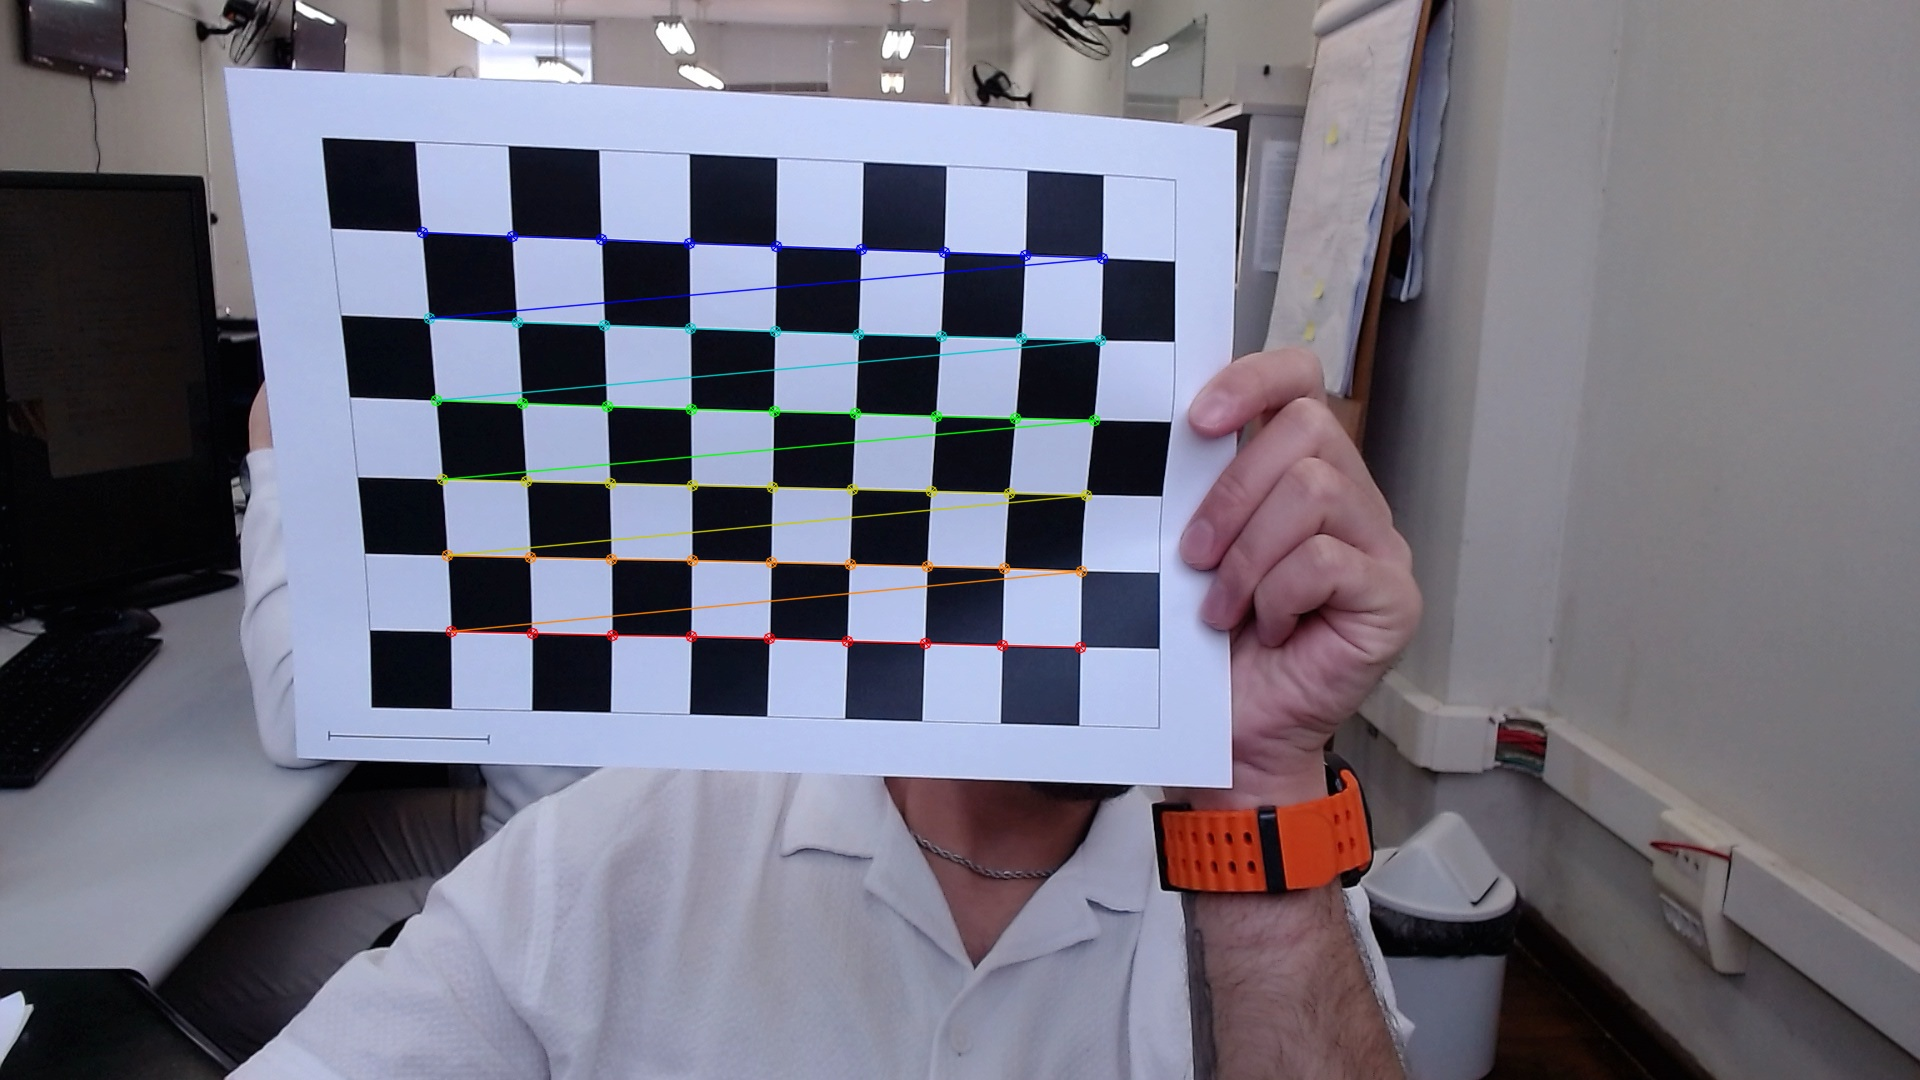
\includegraphics[width=0.88\textwidth]{figuras/cantos_04.jpg}
    \caption{Exemplo de detecção dos 54 cantos internos do padrão de calibração.}
    \label{fig:captura-cantos}
\end{figure}

\section{Calibração intrínseca}
Para cada imagem válida, foram associados os pontos 2D detectados na imagem a um conjunto de pontos 3D conhecidos. Como o padrão é plano, adotou-se $Z=0$, enquanto as coordenadas $X$ e $Y$ foram definidas em milímetros a partir das dimensões reais dos quadrados.

A função \texttt{cv.calibrateCamera()} foi utilizada para estimar a matriz intrínseca, os coeficientes de distorção e os parâmetros extrínsecos referentes a cada pose do tabuleiro.

\section{Correção da distorção}
A correção das imagens foi realizada por meio da função \texttt{cv.undistort()}, utilizando a matriz intrínseca e os coeficientes de distorção obtidos na etapa de calibração. As imagens original e corrigida foram comparadas visualmente, especialmente nas regiões periféricas do quadro.

\section{Experimento de projeção 3D--2D}
Para verificar experimentalmente a projeção geométrica, a pose do tabuleiro em imagens selecionadas foi estimada com \texttt{cv.solvePnP()}. Em seguida, foi definido um cubo virtual de aresta de \SI{50}{\milli\metre} no sistema de coordenadas do tabuleiro.

Os oito vértices do cubo foram projetados para o plano da imagem por meio da função \texttt{cv.projectPoints()}. Para cada vértice, foram registradas as coordenadas tridimensionais $(X,Y,Z)$ e as coordenadas projetadas $(u,v)$ em pixels. Como verificação adicional, pontos pertencentes ao próprio tabuleiro foram reprojetados e comparados às posições detectadas na imagem.

\chapter{RESULTADOS E DISCUSSÃO}
\section{Parâmetros de calibração}
As 30 imagens capturadas tiveram o padrão detectado e foram utilizadas com sucesso na calibração.

A matriz intrínseca obtida foi

\begin{equation}
K =
\begin{bmatrix}
1387{,}4120 & 0 & 799{,}3454 \\
0 & 1367{,}5628 & 544{,}2728 \\
0 & 0 & 1
\end{bmatrix}.
\end{equation}

Os coeficientes de distorção estimados foram

\begin{equation}
 d = [-0{,}007616,\ 0{,}214461,\ -0{,}003646,\ -0{,}034388,\ -0{,}263514].
\end{equation}

O valor RMS retornado pelo processo de calibração foi de 3,6562, coincidindo com o RMSE global de reprojeção de aproximadamente 3,6562 pixels. Considerando as imagens individualmente, o RMSE variou de 2,0297 a 6,2847 pixels, com média de 3,5003 pixels.

\begin{table}[H]
\centering
\caption{Resumo dos parâmetros intrínsecos estimados.}
\label{tab:intrinsecos}
\begin{tabular}{lc}
\toprule
Parâmetro & Valor \\
\midrule
$f_x$ & 1387,4120 px \\
$f_y$ & 1367,5628 px \\
$c_x$ & 799,3454 px \\
$c_y$ & 544,2728 px \\
RMS do OpenCV & 3,6562 \\
RMSE global de reprojeção & 3,6562 px \\
\bottomrule
\end{tabular}
\end{table}

\section{Remoção da distorção}
A Figura~\ref{fig:comparacao-distorcao} apresenta a mesma cena antes e depois da aplicação dos parâmetros de calibração. A correção produz uma alteração visível principalmente nas regiões periféricas, onde a câmera apresenta forte curvatura das linhas. A imagem corrigida também contém regiões pretas sem informação válida, consequência do remapeamento necessário para compensar a distorção e preservar um campo de visão amplo.

\begin{figure}[H]
    \centering
    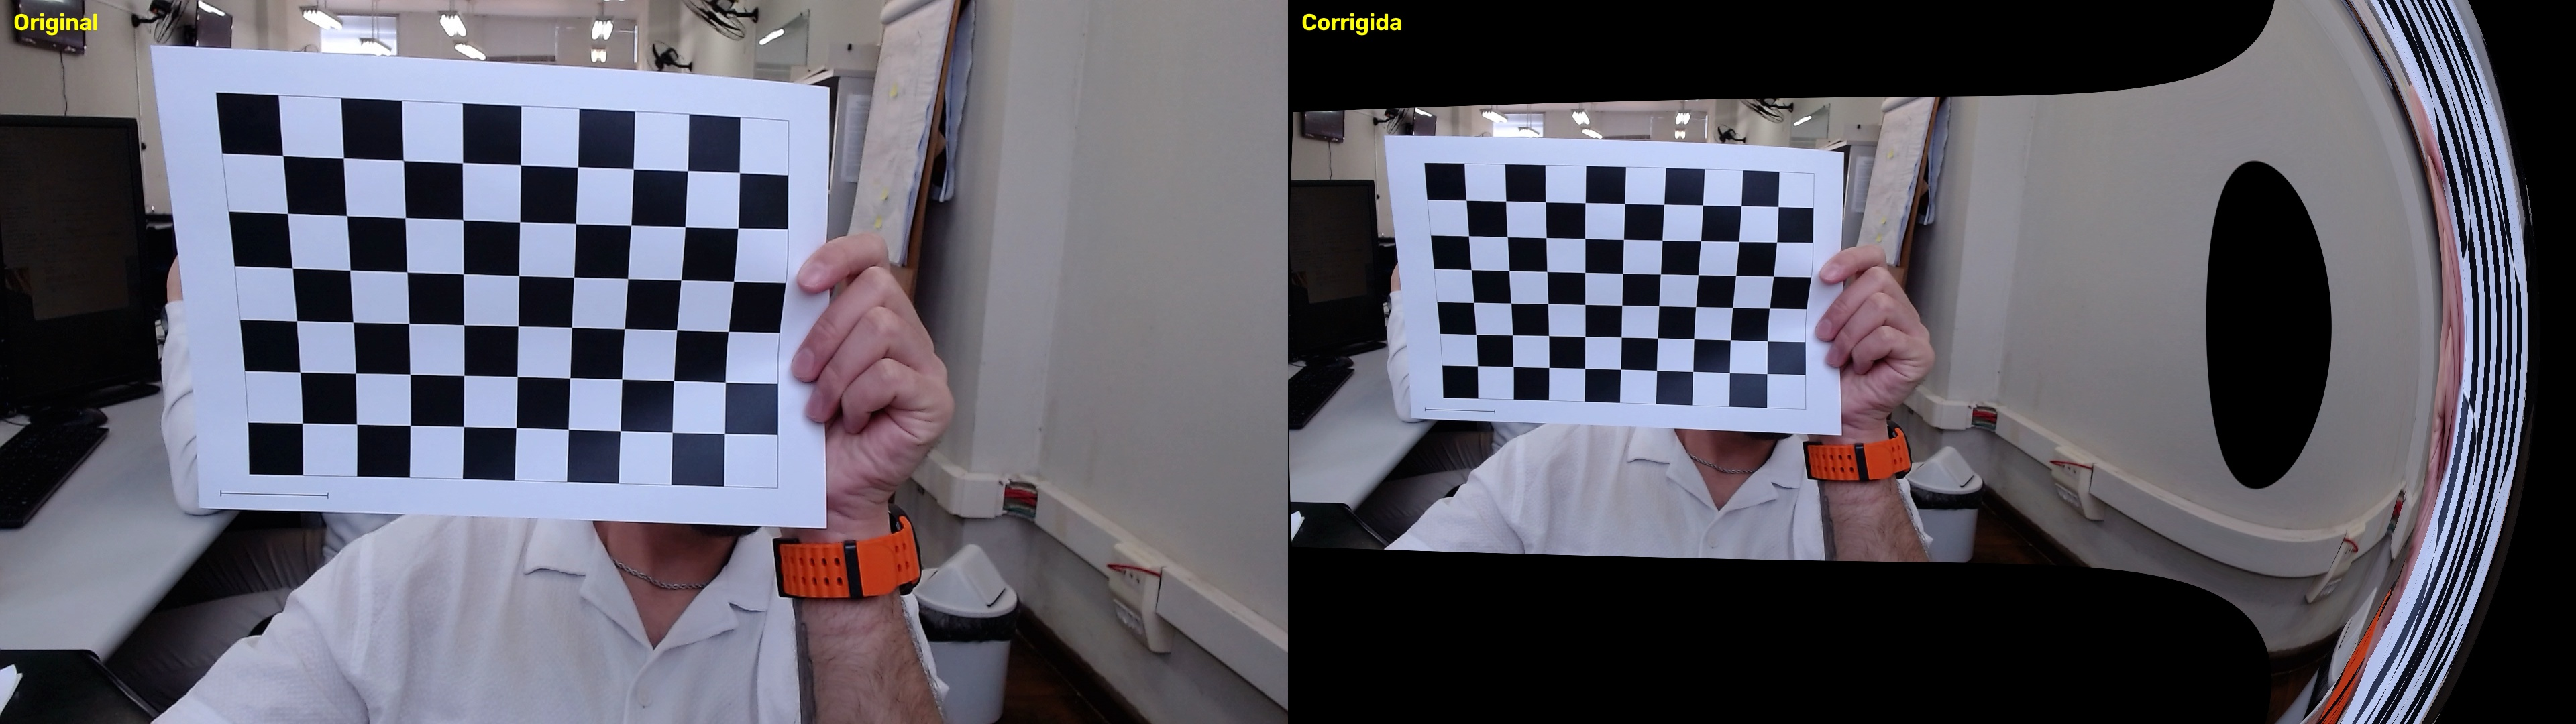
\includegraphics[width=\textwidth]{figuras/distorcao_04.jpg}
    \caption{Comparação entre a imagem original e a imagem após a remoção da distorção.}
    \label{fig:comparacao-distorcao}
\end{figure}

\section{Projeção de pontos tridimensionais}
A projeção foi executada em cinco imagens. A Figura~\ref{fig:cubo-projetado} mostra três poses representativas. Em todas elas, a orientação do cubo acompanha a perspectiva do padrão, fornecendo uma verificação visual da pose estimada e dos parâmetros de calibração.

\begin{figure}[H]
    \centering
    \begin{subfigure}{0.32\textwidth}
        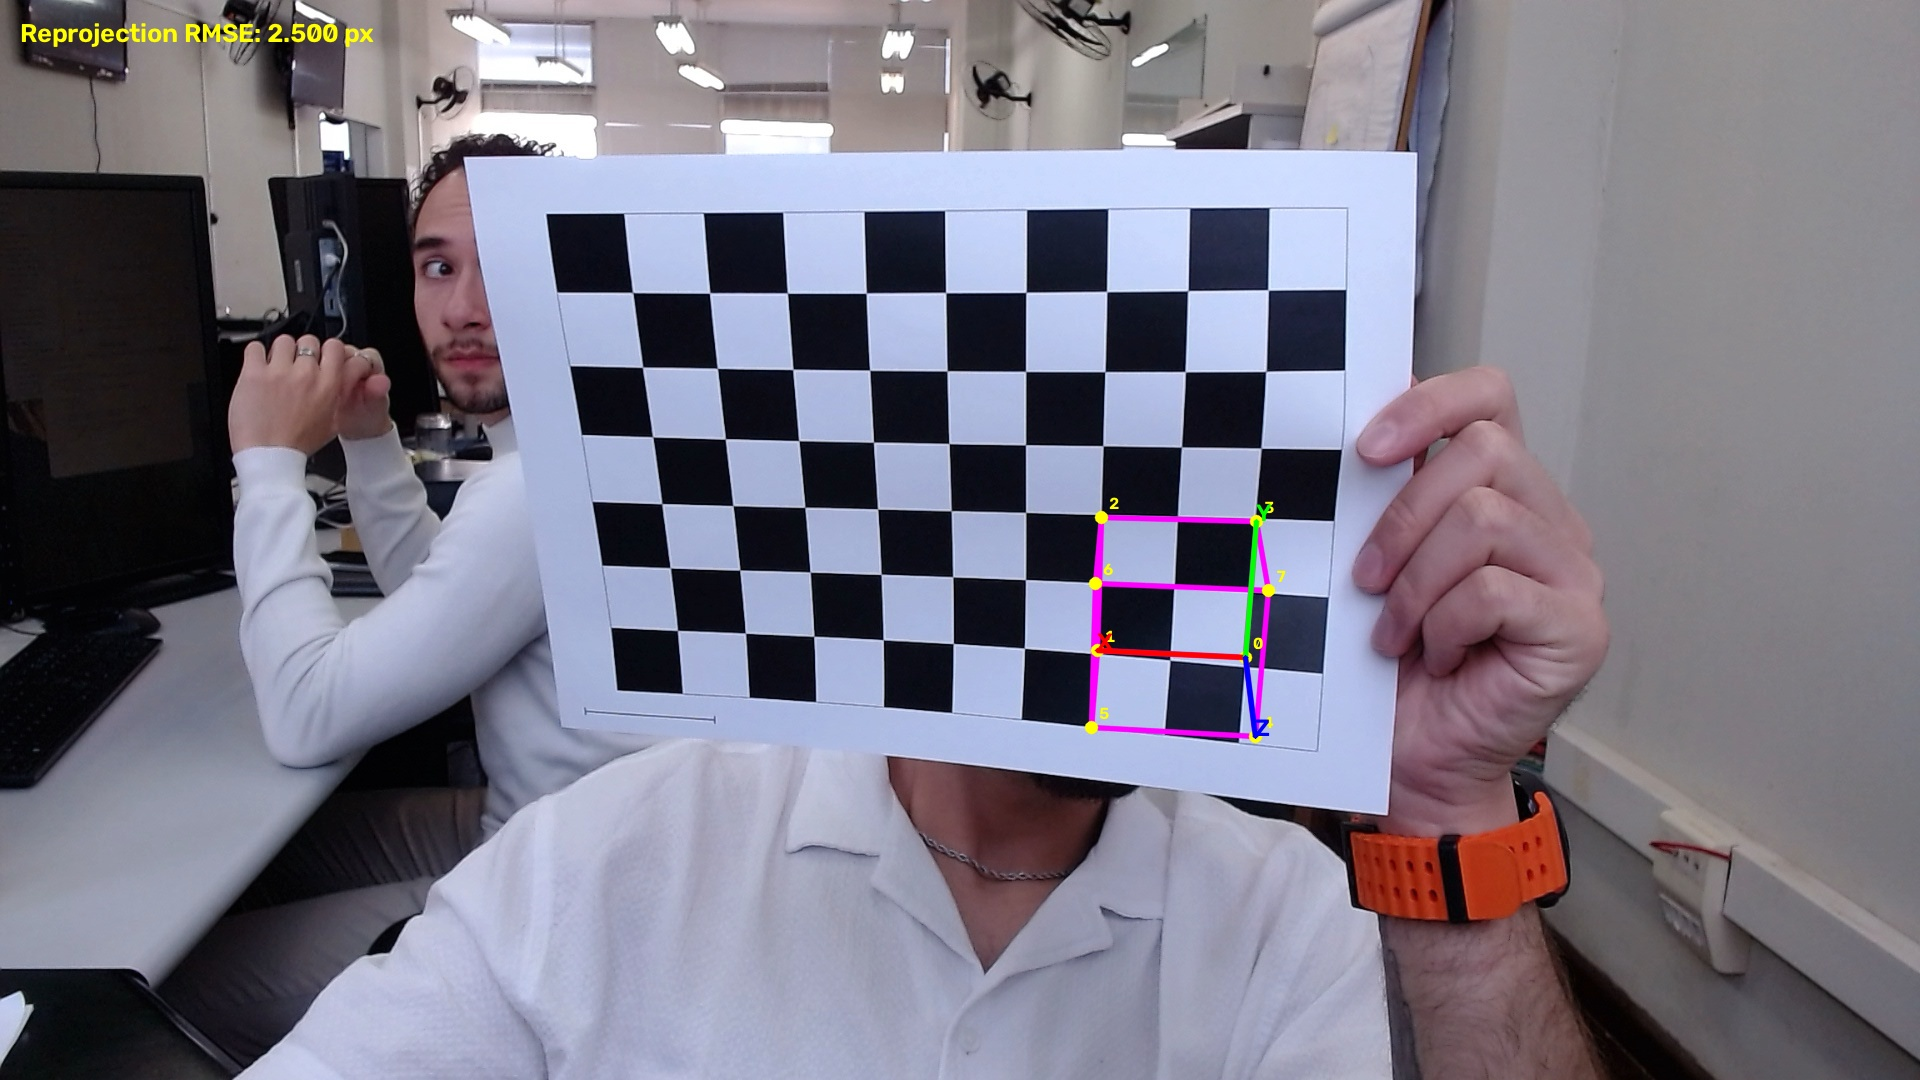
\includegraphics[width=\linewidth]{figuras/projecao_01.jpg}
        \caption{Imagem 01.}
    \end{subfigure}
    \hfill
    \begin{subfigure}{0.32\textwidth}
        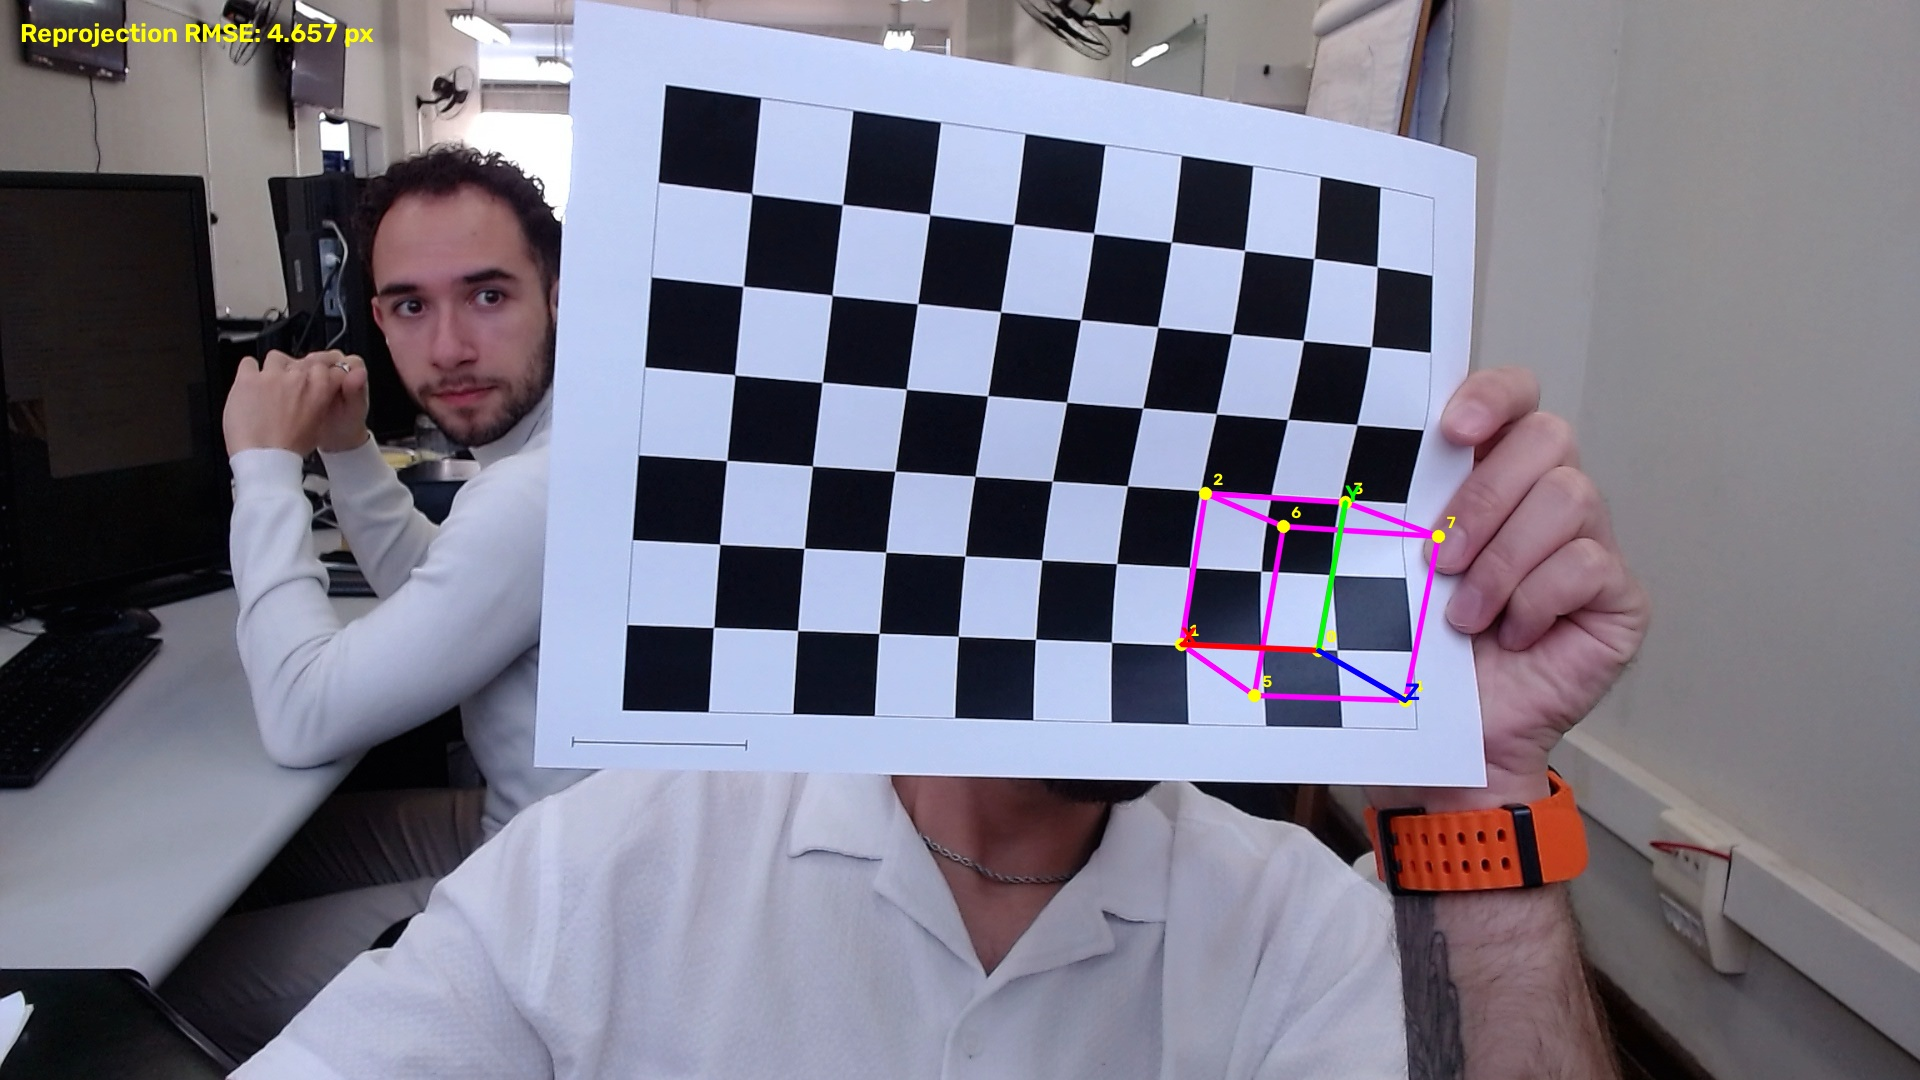
\includegraphics[width=\linewidth]{figuras/projecao_03.jpg}
        \caption{Imagem 03.}
    \end{subfigure}
    \hfill
    \begin{subfigure}{0.32\textwidth}
        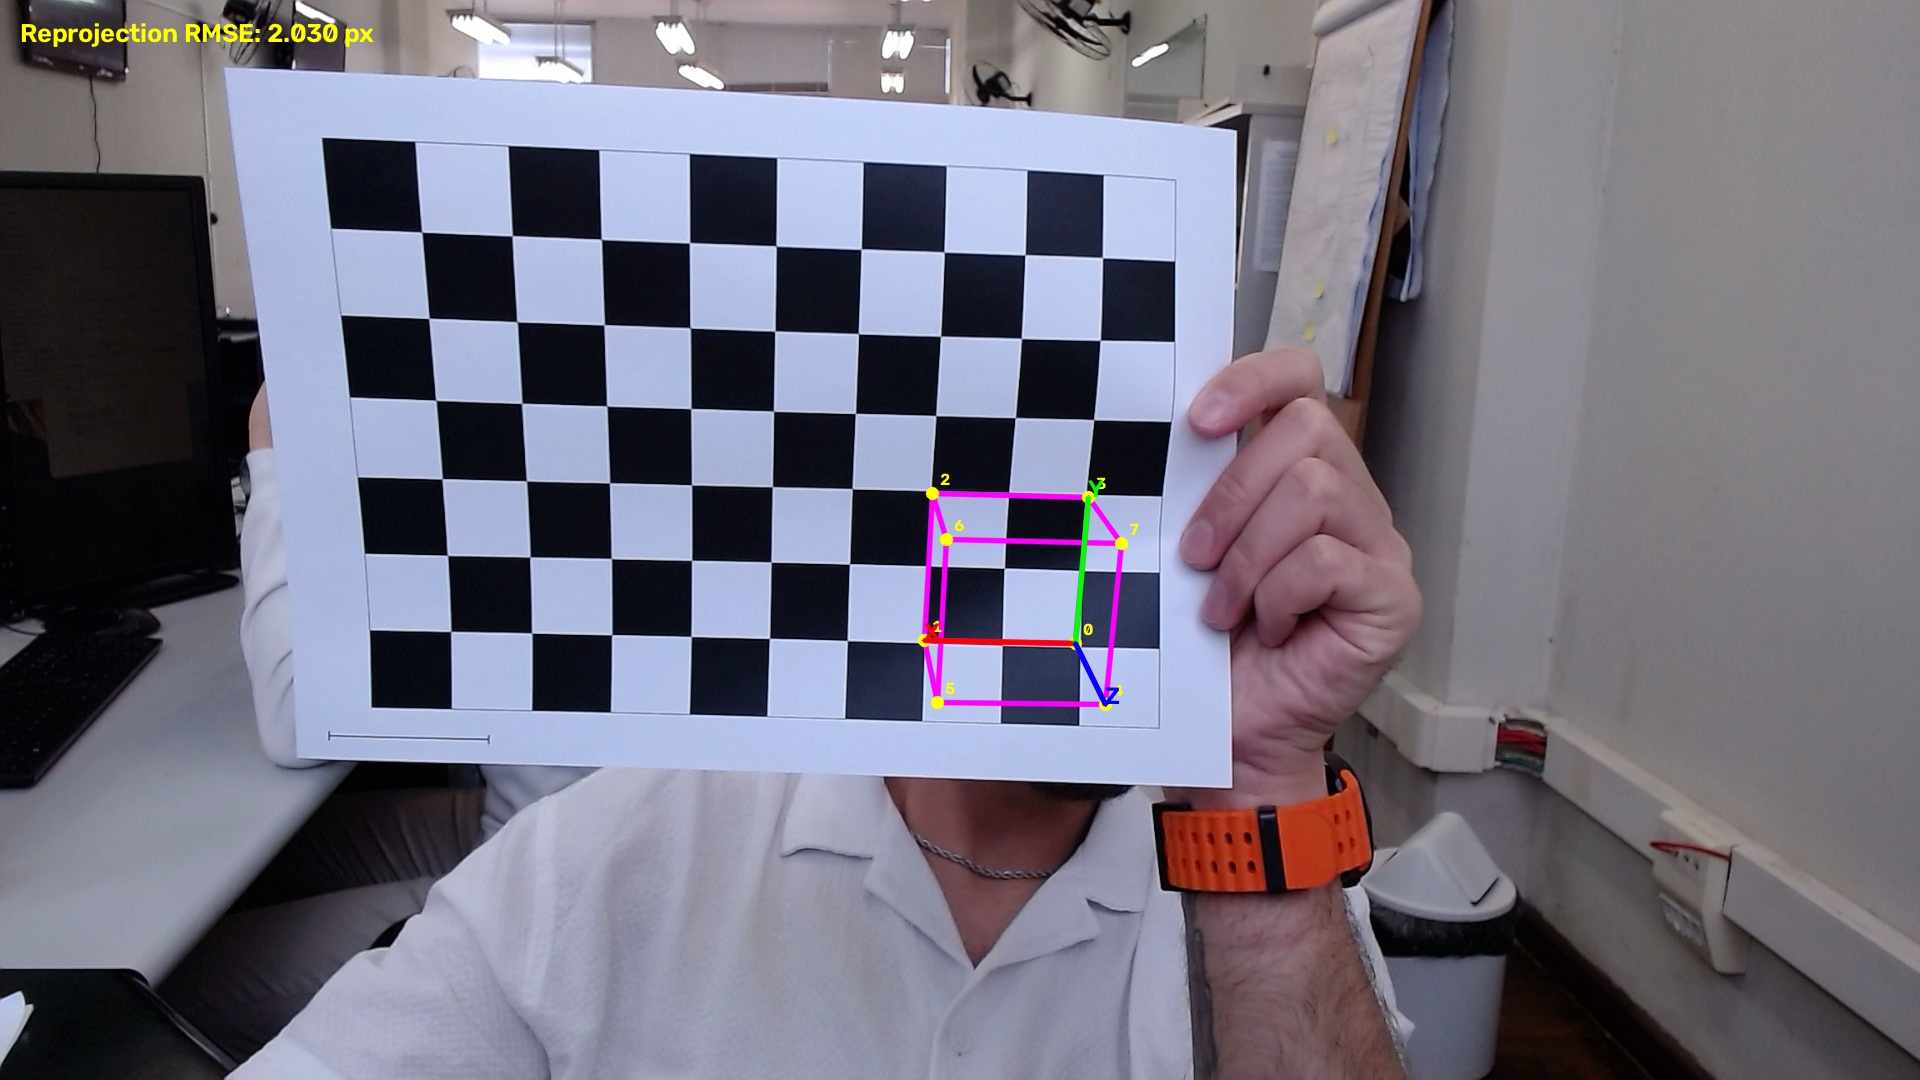
\includegraphics[width=\linewidth]{figuras/projecao_04.jpg}
        \caption{Imagem 04.}
    \end{subfigure}
    \caption{Projeção de um cubo virtual de \SI{50}{\milli\metre} em diferentes poses do padrão.}
    \label{fig:cubo-projetado}
\end{figure}

A Tabela~\ref{tab:projecoes-resumo} resume os erros nas cinco imagens utilizadas no experimento de projeção.

\begin{table}[H]
\centering
\caption{Erro de reprojeção nas cinco imagens do experimento 3D--2D.}
\label{tab:projecoes-resumo}
\begin{tabular}{lcc}
\toprule
Imagem & RMSE (px) & Erro médio (px) \\
\midrule
01 & 2,4999 & 1,9595 \\
02 & 3,7014 & 2,7117 \\
03 & 4,6574 & 3,5904 \\
04 & 2,0297 & 1,6730 \\
05 & 3,1544 & 2,3995 \\
\bottomrule
\end{tabular}
\end{table}

A Tabela~\ref{tab:projecao} apresenta o formato de registro das coordenadas dos vértices projetados.

\begin{table}[H]
\centering
\caption{Coordenadas 3D dos vértices e respectivas projeções na imagem.}
\label{tab:projecao}
\small
\begin{tabular}{cccccc}
\toprule
Ponto & $X$ (mm) & $Y$ (mm) & $Z$ (mm) & $u$ (px) & $v$ (px) \\
\midrule
0 & 0 & 0 & 0 & 1074.98 & 642.83 \\
1 & 50 & 0 & 0 & 924.09 & 640.10 \\
2 & 50 & 50 & 0 & 931.98 & 492.83 \\
3 & 0 & 50 & 0 & 1087.93 & 496.74 \\
4 & 0 & 0 & -50 & 1105.10 & 704.12 \\
5 & 50 & 0 & -50 & 936.65 & 701.55 \\
6 & 50 & 50 & -50 & 946.45 & 538.52 \\
7 & 0 & 50 & -50 & 1121.18 & 542.51 \\
\bottomrule
\end{tabular}
\end{table}

\section{Verificação quantitativa}
Para conferir a projeção, pontos conhecidos do tabuleiro foram comparados com suas respectivas coordenadas calculadas pelo modelo calibrado. O erro euclidiano de cada ponto é dado por

\begin{equation}
 e_i = \sqrt{(u_i-\hat{u}_i)^2 + (v_i-\hat{v}_i)^2},
\end{equation}

em que $(u_i,v_i)$ é a posição detectada e $(\hat{u}_i,\hat{v}_i)$ é a posição reprojetada.

\begin{table}[H]
\centering
\caption{Exemplo de verificação das coordenadas projetadas.}
\label{tab:verificacao}
\small
\begin{tabular}{cccccc}
\toprule
Ponto & $u$ detectado & $v$ detectado & $u$ projetado & $v$ projetado & Erro (px) \\
\midrule
0 & 1080.15 & 646.94 & 1074.98 & 642.83 & 6.60 \\
5 & 691.07 & 636.46 & 691.30 & 635.69 & 0.80 \\
11 & 927.12 & 565.92 & 928.11 & 567.73 & 2.06 \\
17 & 447.39 & 555.33 & 446.47 & 556.73 & 1.67 \\
23 & 691.50 & 484.92 & 691.15 & 486.59 & 1.71 \\
\bottomrule
\end{tabular}
\end{table}

Na imagem 04, utilizada como exemplo por apresentar o menor RMSE entre as cinco imagens de projeção, o RMSE foi de 2,0297 pixels. A maior diferença entre os pontos amostrados ocorreu no canto de índice 0, com aproximadamente 6,60 pixels, enquanto vários pontos internos apresentaram erro inferior a 2 pixels. No conjunto completo de 30 imagens, os maiores erros ocorreram em algumas poses específicas, chegando a 6,2847 pixels de RMSE por imagem. Essas diferenças podem estar associadas à forte distorção da lente nas regiões periféricas, à posição do padrão no quadro, a pequenas deformações da folha impressa e ao ruído subpixel na localização dos cantos. Ainda assim, o cubo projetado permaneceu geometricamente coerente nas diferentes poses testadas.

\chapter{CONCLUSÃO}
Foi realizada a calibração monocular de uma câmera Logitech utilizando um padrão quadriculado e a biblioteca OpenCV. Todas as 30 imagens capturadas foram aproveitadas, resultando em uma matriz intrínseca com $f_x=1387,4120$ px, $f_y=1367,5628$ px, $c_x=799,3454$ px e $c_y=544,2728$ px. O RMSE global de reprojeção foi de 3,6562 pixels.

Os coeficientes estimados permitiram remover visualmente grande parte da distorção da lente, embora o remapeamento tenha produzido regiões sem informação nas bordas da imagem corrigida. No experimento 3D--2D, um cubo de 50 mm foi projetado em cinco imagens por meio da pose estimada com \texttt{solvePnP()} e da função \texttt{projectPoints()}. A projeção acompanhou a perspectiva do tabuleiro e os erros obtidos permitiram conferir quantitativamente a consistência do modelo. Dessa forma, o experimento atendeu aos objetivos de estimar os parâmetros da câmera, corrigir a distorção e verificar a correspondência entre pontos do espaço tridimensional e coordenadas de imagem.

\chapter{REPOSITÓRIO}
O código-fonte, os dados utilizados e os resultados do experimento estão disponíveis em:

\begin{center}
\texttt{\pendente{link do repositório Git}}
\end{center}

\postextual
\begin{thebibliography}{99}

\bibitem{zhang2000}
ZHANG, Zhengyou. A Flexible New Technique for Camera Calibration. \textbf{IEEE Transactions on Pattern Analysis and Machine Intelligence}, v. 22, n. 11, p. 1330--1334, 2000.

\bibitem{opencv_calibration}
OPENCV. \textbf{Camera Calibration}. OpenCV Documentation. Disponível em: \url{https://docs.opencv.org/4.x/dc/dbb/tutorial_py_calibration.html}. Acesso em: 7 out. 2026.

\bibitem{opencv_calib3d}
OPENCV. \textbf{Camera Calibration and 3D Reconstruction}. OpenCV Documentation -- calib3d. Disponível em: \url{https://docs.opencv.org/4.x/d9/d0c/group__calib3d.html}. Acesso em: 7 out. 2026.

\end{thebibliography}
\end{document}
